% Initial version by Darian Muresan, Ph.D.
% dmuresan@stevens.edu
% Edit and adjust as needed.
\documentclass[12pt]{cornell}

% add index support
%\usepackage{imakeidx}
\usepackage{makeidx}

%\makeindex

% graphing programs
\usepackage{color}
\usepackage{psfrag}
\usepackage{verbatim}
\usepackage{fancyhdr}
%\usepackage{titlesec}
\usepackage{fancyvrb} 
% hyperlink programs
%\usepackage{url}

% Does not work with LaTeX=>PDF
\usepackage[pdfmark, 
breaklinks=true, 
colorlinks=true,
citecolor=blue,
linkcolor=blue,
menucolor=black,
pagecolor=black,
urlcolor=blue
]{hyperref} % links in pdf

%\usepackage[colorlinks]{hyperref} % links in dvi
\usepackage{listings}
\usepackage{amsfonts} 
\usepackage{amssymb} 
\usepackage{minted}
%\usepackage{tabto}

\usepackage{tabularx,colortbl}
\usepackage[chapter]{algorithm} 
\usepackage{algorithmic} 
\usepackage{blindtext}

\definecolor{DarkGreen}{rgb}{0,0.6,0}
\definecolor{mygreen}{rgb}{0,0.6,0}
\definecolor{mygray}{rgb}{0.5,0.5,0.5}
\definecolor{mymauve}{rgb}{0.58,0,0.82}

\usepackage{tocloft}
\usepackage{amsmath}
\usepackage{tcolorbox}
\usepackage{enumitem}
\usepackage{longtable}
%\usepackage{textcomp}
\usepackage{txfonts}
\usepackage{pstool}

%part for \part titles
%chap for \chapter titles
%sec for \section titles
%subsec for \subsection titles
%subsubsec for \subsubsection titles
%para for \paragraph titles
%subpara for \subparagraph titles
%fig for figure \caption titles
%subfig for subfigure \caption titles
%tab for table \caption titles
%subtab for subtable \caption titles


% update chapter number spacing
\setlength{\cftchapnumwidth}{2em}
\setlength{\cftsecnumwidth}{2.5em}
\setlength{\cftsubsecnumwidth}{3.5em}
\setlength{\cftsubsubsecnumwidth}{4.5em}

\addtolength{\cftsecindent}{0.5em}
\addtolength{\cftsubsecindent}{0.5em}
\addtolength{\cftsubsubsecindent}{0.5em}

%\titlespacing*{\chapter}{0pt}{-50pt}{20pt}
%\titleformat{\chapter}[display]{\normalfont\huge\bfseries}{\chaptertitlename\ 
%\thechapter}{20pt}{\Huge}
%\pagestyle{fancy}
%\pagestyle{cornell}
%
%\rhead{F054-021-0172}
%\chead{Nonlinear Enhancement of Visual Target Detection (AF05-T021)}
%\lhead{GSTI}
%\lfoot{\scriptsize Use or disclosure of data on this page is subject
%to the restriction on the title page of this proposal.}
%\cfoot{}
%\rfoot{\thepage}

\newfont{\Bp}{msbm10}
\newfont{\BpBig}{msbm10 scaled\magstep2}
\newfont{\Sc}{eusm10}
\newfont{\ScBig}{eusm10 scaled\magstep3}
\newfont{\Fr}{eufm10}
\newfont{\FrBig}{eufm10 scaled\magstep1}

% some commands:
\newcommand{\dxi}{{\tt m\_xDeltaInput}}
\newcommand{\dyi}{{\tt m\_yDeltaInput}}
\newcommand{\dci}{{\tt m\_cDeltaInput}}
\newcommand{\dxo}{{\tt m\_xDeltaOutput}}
\newcommand{\dyo}{{\tt m\_yDeltaOutput}}
\newcommand{\dco}{{\tt m\_cDeltaOutput}}
\newcommand{\ttf}[1]{{\tt #1}}
\newcommand{\tbl}[2]{{\begin{tabular}{c} #1 \\ #2 \end{tabular}}}

\newcommand{\urltwo}[2]{\mbox{\href{#1}{\tt #2}}}
\newcommand{\qnorm}[1]{\|#1\|_{\bQ}}
\newcommand{\qdot}[2]{\lrb #1, #2 \rrb_{\bQ}}
\newcommand{\kdot}[2]{\lrb #1, #2 \rrb_{\bf k}}
\newcommand{\tdot}[2]{\lrb #1, #2 \rrb}
\newcommand{\mydiff}[2]{\lrb #1 - #2 \rrb}
\newcommand{\lena}{\textit{lena}}
\newcommand{\barb}{\textit{barbara}}
\newcommand{\boat}{\textit{boat}}
\newcommand{\leaves}{\textit{leaves}}
\newcommand{\rings}{\textit{rings}}
\newcommand{\treg}{\textit{train region}}
\newcommand{\dreg}{\textit{denoise region}}
\newcommand{\oreg}{\textit{overlap region}}
\newcommand{\sil}{\sigma_l^2}
\newcommand{\sn}{\sigma^2}
\newcommand{\bn}{{\mbox{\bf \FrBig N}}}
\newcommand{\n}{\mbox{\Fr N}}
%\newcommand{\bn}{\bf N}
%\newcommand{\n}{N}
\newcommand{\bY}{\textbf{Y}}
\newcommand{\bX}{\textbf{X}}
\newcommand{\bb}{\textbf{b}}
\newcommand{\bu}{\textbf{u}}
\newcommand{\bv}{\textbf{v}}
\newcommand{\by}{\textbf{y}}
\newcommand{\bx}{\textbf{x}}
\newcommand{\be}{\textbf{e}}
\newcommand{\bz}{\textbf{z}}
\newcommand{\bs}{\textbf{s}}
\newcommand{\bw}{\textbf{w}}
\newcommand{\bQ}{\textbf{Q}}
\newcommand{\bphi}{\textbf{$\phi$}}
\newcommand{\lsb}{\left[}
\newcommand{\rsb}{\right]}
\newcommand{\lrb}{\left(}
\newcommand{\rrb}{\right)}
\newcommand{\lcb}{\left\{}
\newcommand{\rcb}{\right\}}
\newcommand{\R}{\mbox{\BpBig R}}
\newcommand{\F}{{\cal F}}
\newcommand{\Fk}{\mbox{\Sc F}}
\newcommand{\bQF}{\textbf{Q}_{\mbox{\Sc F}}}
\newcommand{\N}{{\cal N}}
\newcommand{\xlz}{X_l(z)}
\newcommand{\xhz}{X_h(z)}
\newcommand{\xz}{X(z)}
\newcommand{\pr}{ perfect reconstruction }
\newcommand{\smb}{Smith-Barnwell }
\newcommand{\xw}{X(e^{j\omega})}
\newcommand{\xmw}{X(-e^{j\omega})}
\newcommand{\dw}{D(e^{j\omega})}
\newcommand{\dmw}{D(-e^{j\omega})}
\newcommand{\ew}{E(e^{j\omega})}
\newcommand{\emw}{E(-e^{j\omega})}
\newcommand{\fw}{F_0(e^{j\omega})}
\newcommand{\fmw}{F_0(-e^{j\omega})}
\newcommand{\hoz}{H_1(z)}
\newcommand{\hzz}{H_0(z)}
\newcommand{\goz}{G_1(z)}
\newcommand{\gzz}{G_0(z)}
\newcommand{\hzw}{H_{0}(e^{j\omega})}
\newcommand{\hzmw}{H_{0}(-e^{j\omega})}
\newcommand{\hzcw}{H_{0}(e^{-j\omega})}
\newcommand{\how}{H_1(e^{j\omega})}
\newcommand{\homw}{H_1(-e^{j\omega})}
\newcommand{\gzw}{G_0(e^{j\omega})}
\newcommand{\gzmw}{G_0(-e^{j\omega})}
\newcommand{\gow}{G_1(e^{j\omega})}
\newcommand{\gomw}{G_1(-e^{j\omega})}
\newcommand{\wl}{e^{-jwL}}
\newcommand{\aqua}{\textit{AQua with OR }}
\newtheorem{theorem}{Theorem}
\newtheorem{lemma}{Lemma}
\newtheorem{corollary}{Corollary}
\newtheorem{claim}{Claim}
\newtheorem{definition}{Definition}
\newenvironment{proof}{\noindent{\em Proof.}}{\ \hfill Q.E.D.}
%\newtheorem{moduleCount}{L}
\newcommand*{\labelfile}[1]{%
  \label{file:#1}%
}

% Use this to label requirements, use cases, user stories, etc.
% This is where we can add different spellings for different types of 
% requirements, use cases, user stories, etc.
% \newtheorem{requirementKind}{Requirement Spelling}
\newtheorem{reqkFunctional}{Functional Requirement}
\newtheorem{reqkQuality}{Quality Requirement}
\newtheorem{reqkConstraint}{Constraint Requirement}
\newtheorem{reqkInterface}{Interface Requirement}
\newtheorem{reqkBusiness}{Business Requirement}
% Use cases
\newtheorem{useCase}{Use Case}
% User story
\newtheorem{userStory}{User Story}

% command for adding a version to the document
\newcommand{\VERSION}{Version 0.0.0}

% Family -- enter the name of the family that it belongs to: Chapter, Figure, Table, etc.
% Name -- name of the family member: file name, table name, etc.
\newcommand{\FamilyName}[2]{\hyperref[#1::#2]{#2}\index{#2}\xspace}
% Family -- same as above
% Name -- same as above
% Reference -- shorthand for the 'Name'.  It will show as Reference_NameID
% Kind -- underscore(_), space, or dash (-)
\newcommand{\FamilyNameReferenceKind}[4]{\hyperref[#1::#2]{$#3#4{\ref*{#1::#2}}$}}
% newcommand{Family,Label}
\newcommand{\FamilyLabel}[2]{\label{#1::#2}}


% for use cases
\newcommand{\UseCaseLabel}[1]{\FamilyLabel{UseCase}{#1}}
\newcommand{\UseCaseName}[1]{\FamilyName{UseCase}{#1}}
\newcommand{\UseCaseReference}[1]{\FamilyNameReferenceKind{UseCase}{#1}{UC}{_}}
% UseCase name with stacked reference
\newcommand{\UseCaseNameWSReference}[1]{\begin{tabular}{c}\UseCaseName{#1} \\ (\UseCaseReference{#1}) \end{tabular}}
% UseCase name with inline reference
\newcommand{\UseCaseNameWIReference}[1]{\UseCaseName{#1} (\UseCaseReference{#1})}

% for chapters
\newcommand{\ChapterName}[1]{\FamilyName{Chapter}{#1}}
\newcommand{\ChapterLabel}[1]{\FamilyLabel{Chapter}{#1}}
\newcommand{\ChapterReference}[1]{\FamilyNameReferenceKind{Chapter}{#1}{Chapter}{\mbox{ }}}
% Chapter name with inline (WI) reference 
\newcommand{\ChapterNameWIReference}[1]{\ChapterName{#1} (\ChapterReference{#1})}

% for figures
\newcommand{\FigureName}[1]{\FamilyName{Figure}{#1}}
\newcommand{\FigureLabel}[1]{\FamilyLabel{Figure}{#1}}
\newcommand{\FigureReference}[1]{\FamilyNameReferenceKind{Figure}{#1}{Figure}{\mbox{ }}}
% Figure name with stacked (WS) reference
\newcommand{\FigureNameWSReference}[1]{\begin{tabular}{c}\FigureName{#1} \\ (\FigureReference{#1}) \end{tabular}}
% Figure name with inline (WI) reference 
\newcommand{\FigureNameWIReference}[1]{\FigureName{#1} (\FigureReference{#1})}

% for tables
\newcommand{\TableName}[1]{\FamilyName{Table}{#1}}
\newcommand{\TableLabel}[1]{\FamilyLabel{Table}{#1}}
\newcommand{\TableReference}[1]{\FamilyNameReferenceKind{Table}{#1}{Table}{\mbox{ }}}

% for requirements
% RequirementLabel[Kind][Label]
\newcommand{\RequirementLabel}[2]{\FamilyLabel{#1}{#2}}
\newcommand{\RequirementName}[2]{\FamilyName{#1}{#2}}
\newcommand{\RequirementReference}[2]{\FamilyNameReferenceKind{#1}{#2}{#1}{_}}
% Requirements name with stacked (WS) reference
\newcommand{\RequirementNameWSReference}[2]{\begin{tabular}{c}\RequirementName{#1}{#2} \\ (\RequirementReference{#1}{#2}) \end{tabular}}
% Requirements name with inline (WI) reference 
\newcommand{\RequirementNameWIReference}[2]{\RequirementName{#1}{#1} (\RequirementReference{#1}{#2})}

% for requirements
% RequirementLabel[Kind][Label]
\newcommand{\UserStoryLabel}[2]{\FamilyLabel{#1}{#2}}
\newcommand{\UserStoryName}[2]{\FamilyName{#1}{#2}}
\newcommand{\UserStoryReference}[2]{\FamilyNameReferenceKind{#1}{#2}{R}{_}}
% Requirements name with stacked (WS) reference
\newcommand{\UserStoryNameWSReference}[2]{\begin{tabular}{c}\RequirementName{#1}{#2} \\ (\RequirementReference{#1}{#2}) \end{tabular}}
% Requirements name with inline (WI) reference 
\newcommand{\UserStoryNameWIReference}[2]{\RequirementName{#1}{#1} (\RequirementReference{#1}{#2})}



\lstset{ %
  backgroundcolor=\color{white},   % choose the background color; you must add \usepackage{color} or \usepackage{xcolor}
  basicstyle=\footnotesize,        % the size of the fonts that are used for the code
  breakatwhitespace=false,         % sets if automatic breaks should only happen at whitespace
  breaklines=true,                 % sets automatic line breaking
  captionpos=b,                    % sets the caption-position to bottom
  commentstyle=\color{DarkGreen},    % comment style
  deletekeywords={...},            % if you want to delete keywords from the given language
  escapeinside={\%*}{*)},          % if you want to add LaTeX within your code
  extendedchars=true,              % lets you use non-ASCII characters; for 8-bits encodings only, does not work with UTF-8
  %frame=single,                   % adds a frame around the code
  keepspaces=true,                 % keeps spaces in text, useful for keeping indentation of code (possibly needs columns=flexible)
  keywordstyle=\color{blue},       % keyword style
  language=C++,                    % the language of the code
  morekeywords={*,...},            % if you want to add more keywords to the set
  numbers=left,                    % where to put the line-numbers; possible values are (none, left, right)
  numbersep=5pt,                   % how far the line-numbers are from the code
  numberstyle=\tiny\color{mygray}, % the style that is used for the line-numbers
  rulecolor=\color{black},         % if not set, the frame-color may be changed on line-breaks within not-black text (e.g. comments (green here))
  showspaces=false,                % show spaces everywhere adding particular underscores; it overrides 'showstringspaces'
  showstringspaces=false,          % underline spaces within strings only
  showtabs=false,                  % show tabs within strings adding particular underscores
  stepnumber=1,                    % the step between two line-numbers. If it's 1, each line will be numbered
  stringstyle=\color{mymauve}     % string literal style
  %tabsize=2,                      % sets default tabsize to 2 spaces
  %caption=\lstname                % show the filename of files included with \lstinputlisting; also try caption instead of title
}


% Uncomment draftcopy to get the word DRAFT boldly across the first page
%   By the way, xdvi won't show it but it will come out when you print
%\usepackage[light,all]{draftcopy}		% DRAFT on first page
%\draftcopySetGrey{.97}
%\draftcopyName{Confidential}{150}
%\draftcopFirstPage{1}

% Uncomment drafthead to get the date and DRAFT in the header of pages
% that are normallly numbered on the top, pages 2-n of each chapter for example
% This doesn't work with centered page numbers: \pagestyle{cornellc}
%\usepackage{drafthead}

% glossaries to organize the document glossary
%\usepackage[toc,chapter,numberedchapter = autolabel]{glossaries}
\usepackage{glossaries}

% glossary creation
\newglossaryentry{must}
{	name={MustHave},
	description={This defines the first highest priority requirement.
	All of the tasks, requirements, or anything that is marked this way are
	build in the current version}
}

\newglossaryentry{should}
{	name={ShouldHave},
	description={This defines the second highest priority requirement. The system should implement 
	all of the tasks, requirements, or anything that is marked this way, but if 
	resources are limited, it can be left out of the current version.
	Build in next version}
}

\newglossaryentry{could}
{	name={CouldHave},
	description={This defines the third highest priority requirement.The system could implement 
	all of the tasks, requirements, or anything that is marked this way, but if 
	resources are limited, it can be left out of the current and next version.
	Build in two versions from now}
}

\newglossaryentry{would}
{	name={WouldHave},
	description={This defines the lowest priority requirement.  The system would like to implement 
all of the tasks, requirements, or anything that is marked this way, but only
if resources are available. It can be left out of all future versions}
}

%\makeglossaries
\makenoidxglossaries
\makeindex

% Including selective chapters:
% use this to selectively process chapters, etc.  Put a % in front of
% the sections that you don't want done this time.  Includes are
% used instead of \input so that LaTeX will keep track of chapters and
% pages without processing everything.  Don't let any spaces creep in
% around the words or it will not work!

\includeonly{
prologue,
itIntroduction,
itPasswords,
itHosts,
itLinuxCommands,
itAppendix,
itprojectproposal,
itAWSDeployment,
itLaTeXDocker,
itBugzilla,
itOverleaf,
itOverleafGithub
}


\begin{document}

\pagenumbering{roman}
\singlespacing
% File: prologue.tex
% Thesis prologue:  Title page, acknowledgements, table of contents,
% list of figures, and list of tables.
%
% this file is to be \include'd after the \begin{document}

% Cornell-style title page
\begin{titlepage}
        \title{SSW 590}
        \author{Ivan Farfan, Johan Jaramillo, Ryan Davis \\ Stevens.edu }
        \conferraldate{}{\today} \maketitle
\end{titlepage}

% Copyright page
%\begin{copyrightpage}
\makecopyright
%\end{copyrightpage}

% Abstract: the abstract body is pulled from the file abstract.tex;
%  the title is pulled from the \title command in the titlepage section
\begin{abstract}
        %\makeabstitle
        \input abstract      % puts the abstract file here
\end{abstract}

% Biographical information pulled from file bio.tex
%\begin{biosketch} \input bio \end{biosketch}

% Dedication (optional):  pulls information from file dedication.tex
%\begin{dedication} 
%\input dedicate 
%\end{dedication}

% Acknowledgements:  pulls information from file acknow
%\begin{acknowledgements} \input acknow \end{acknowledgements}

% Table of contents
\contentspage

% If you have no tables or figures put a % in front of the list page line
% List of tables
\tablelistpage

% List of figures
\figurelistpage

\setcounter{page}{1}        % set page counter
\pagenumbering{arabic}      % set page number style
\pagestyle{fancy}         % top right page numbers
%\pagestyle{cornell}
%\pagestyle{cornellc}       % centered page numbers, disables drafthead

\renewcommand{\chaptermark}[1]{\markboth{#1}{}}
\renewcommand{\sectionmark}[1]{\markright{#1}{}}

\fancyhead{} % clear all fields

\lhead{Chapter \thechapter}
%\lhead{\thechapter}
\chead{\leftmark}
\rhead{\thepage}


\lfoot{Chapter \thechapter}
\cfoot{\copyright Stevens -- \today \mbox{} -- Do Not Distribute!}
\rfoot{\thepage}

\renewcommand{\headrulewidth}{0.4pt}
\renewcommand{\footrulewidth}{0.4pt}

%\rhead{F054-021-0172}
%\chead{Nonlinear Enhancement of Visual Target Detection (AF05-T021)}
%\lhead{GSTI}
%\lfoot{\scriptsize Use or disclosure of data on this page is subject
%to the restriction on the title page of this proposal.}
%\cfoot{}
%\rfoot{\thepage}


\singlespacing
\chapter{Kanban Setup \\
\small{\textit{-- Ivan Farfan Diaz, Johan Jaramillo}}
\index{Kanban Setup} 
\index{Chapter!Kanban Setup}
\label{Chapter::Kanban Setup}}

In order to setup our Kanban board, we used Github Projects. The process consisted on:

\begin{enumerate}
    \item \textbf{Creating a Project} -- Going to our repository, clicking ``Projects'' tab, then ``New project''
    
    \item \textbf{Choosing a Template} -- Selecting ``Board'' or ``Kanban'' template (or starting from scratch)
    
    \item \textbf{Setting Up Columns} -- Creating workflow columns like ``To Do,'' ``In Progress,'' ``In Review,'' ``Done''
    
    \item \textbf{Configuring Settings} -- Naming our project, adding description, setting visibility (public/private)
    
\end{enumerate}
\chapter{Passwords \\
\small{\textit{-- Ivan Farfan, Johan Jaramillo, Ryan Davis}}}
\index{Passwords} 
\index{Chapter!Passwords}
\label{Chapter::Passwords}
 
\begin{longtable}{|p{3cm}|p{13cm}|}
\hline
\textbf{Category} & \textbf{Password Rule} \\
\hline
\endfirsthead

\hline
\textbf{Category} & \textbf{Password Rule} \\
\hline
\endhead

% ---------- Server Rules ----------
Server Rules & 
\begin{itemize}
    \item We use a prefix for the site (which city the server is in), then a descriptive shorthand for what the server does. 
    \item Example: \texttt{XXFS01} would be a file server in location \texttt{XX}. 
    \item If there were a second file server in the same location, it would be named \texttt{XXFS02}.
\end{itemize} \\
\hline

% ---------- User Rules ----------
User Rules & 
\begin{itemize}
    \item Passwords must be changed every 60 days.
    \item Users cannot reuse the last 4 passwords.  
    \item Accounts will be locked after 3 failed login attempts.
\end{itemize} \\
\hline

% ---------- General Rules ----------
General Rules & 
\begin{itemize}
    \item Passwords must have at least 10 characters.
    \item Passwords must include at least one uppercase letter.
    \item Passwords must include at least one lowercase letter.
    \item Passwords must include at least one special character (e.g., !, @, \#, \$).
\end{itemize} \\
\hline

% ---------- Custom Rule ----------
Custom Rule & 
\begin{itemize}
    \item Include the abbreviation of the operating system you use. 
    \item Finish with a memorable number, such as the year of graduation or the current semester.
\end{itemize} \\
\hline



% ---------- Digital Ocean ----------
Digital Ocean & 
\begin{itemize}
    \item Follows the standardized password pattern:
    \begin{center}
        \texttt{<coursetag><coursenumber><termLetter>@<serviceInitials>}
    \end{center}
    \item The initials \texttt{do} represent DigitalOcean.
    \item This ensures service-specific uniqueness across all deployed systems.
\end{itemize} \\
\hline

\end{longtable}



\section*{Hints}
\begin{itemize}
    \item User passwords often mix in course codes, semesters, or graduation years. 
    \item General passwords follow the 10+ character, uppercase, lowercase, and special character requirements. 
    \item Custom group passwords contain a Mac/OS reference combined with a number tied to student life.
\end{itemize}
\chapter{Hosts \\
\small{\textit{-- Ivan Farfan, Johan Jaramillo, Ryan Davis}}}
\index{Hosts} 
\index{Chapter!Hosts}
\label{Chapter::Hosts}

This chapter lists the primary hosts used for the project deployment.  
Each host represents a service or container deployed within the shared DigitalOcean environment.  
IP addresses and configurations are specific to the development setup for Fall 2025.


\begin{longtable}{|p{4cm}|p{4cm}|p{3cm}|p{6cm}|}
\caption{Project Hosts and Roles} \label{tab:hosts} \\
\hline
\textbf{Hostname / Service} & \textbf{IP Address} & \textbf{Operating System} & \textbf{Role / Purpose} \\
\hline
\endfirsthead

\multicolumn{4}{c}%
{{\bfseries \tablename\ \thetable{} -- continued from previous page}} \\
\hline
\textbf{Hostname / Service} & \textbf{IP Address} & \textbf{Operating System} & \textbf{Role / Purpose} \\
\hline
\endhead

\hline \multicolumn{4}{|r|}{{Continued on next page}} \\ \hline
\endfoot

\hline
\endlastfoot

Overleaf Container & 167.71.181.60 & Ubuntu 25.04 & Overleaf LaTeX Toolkit deployed via Docker; provides collaborative document editing capabilities. \\
\hline
Bugzilla Container & 167.71.179.151 & Ubuntu 25.04 & Bugzilla issue tracking system deployed in a Docker container for project management and defect tracking. \\
\hline
DigitalOcean Droplet & N/A & Ubuntu 25.04 & Cloud infrastructure host running both the Overleaf and Bugzilla containers within the same droplet environment. \\
\hline
Local Overleaf & ssw590f25.me & Nginx and Ubuntu 25.04 & Public domain that runs our local overleaf version. \\

\end{longtable}


\chapter{Linux Commands \\
\small{\textit{-- Ivan Farfan, Johan Jaramillo, Ryan Davis}}}
\index{Linux Commands} 
\index{Chapter!Linux Commands}
\label{chap:linux}

\section*{Environment Setup}
The following bash commands were executed in a Linux terminal to create the test environment:

\begin{lstlisting}[language=bash]
mkdir -p ~/lx-test && cd ~/lx-test
printf "alpha\nbeta\nGamma\ngamma\nbeta\n" > words.txt
printf "id,name,dept\n1,Ada,EE\n2,Linus,CS\n3,Grace,EE\n4,Dennis,CS\n" > people.csv
printf "INFO boot ok\nWARN disk low\nERROR fan fail\nINFO shutdown\n" > sys.log
dd if=/dev/zero of=blob.bin bs=1K count=48 status=none
mkdir -p src/lib tmp archive
printf "one two three four\n" > src/file1.txt
printf "two three four five\n" > src/file2.txt
ln -s src/file1.txt link-to-file1
touch -t 202401020304 old.txt
\end{lstlisting}

\section*{A) Navigation \& File Ops}
\begin{enumerate}
\item Show your present working directory path only. \vspace{2em}\\
\begin{lstlisting}[language=sh]
    pwd
    /senior_year/ssw590-devops/hw/linuxCommands/lx-test

\end{lstlisting}

\item List all entries in the current directory, one per line, including dotfiles. \vspace{2em}\\
\begin{lstlisting}[language=sh]
ls -a1
    .
    ..
    archive
    blob.bin
    link-to-file1
    old.txt
    people.csv
    src
    sys.log
    tmp
    words.txt

\end{lstlisting}

\item Copy src/file1.txt to tmp/ only if tmp exists; do it verbosely. \vspace{2em}\\
\begin{lstlisting}[language=sh]
[ -d tmp ] && cp -v src/file1.txt tmp/
    src/file1.txt -> tmp/file1.txt
\end{lstlisting}
\item Move old.txt into archive/ and keep its original timestamp. \vspace{2em}\\
\begin{lstlisting}[language=sh]
cp -p old.txt archive/ && rm old.txt

\end{lstlisting}
\item Create a new empty file notes.md only if it doesn’t already exist. \vspace{2em}\\
\begin{lstlisting}[language=sh]
touch -c newfile.txt

\end{lstlisting}
\item Show disk usage (human-readable) for the src directory only (not total FS). \vspace{2em}\\
\begin{lstlisting}[language=sh]
    du -sh src

8.0K	src
\end{lstlisting}
\end{enumerate}

\section*{B) Viewing \& Searching}
\begin{enumerate}
\setcounter{enumi}{6}
\item Print line numbers while displaying sys.log. \vspace{2em}\\
\begin{lstlisting}[language=sh]
nl -ba sys.log

     1	INFO boot ok
     2	WARN disk low
     3	ERROR fan fail
     4	INFO shutdown

\end{lstlisting}

\item Show only the lines in sys.log that contain ERROR (case-sensitive). \vspace{2em}\\
\begin{lstlisting}[language=sh]
cat sys.log|grep ERROR
    ERROR fan fail
\end{lstlisting}
\item Count how many distinct words appear in words.txt (case-insensitive). \vspace{2em}\\
\begin{lstlisting}[language=sh]
tr -c '[:alnum:]' '[\n*]' < words.txt | tr '[:upper:]' '[:lower:]' | sort | uniq | wc -l

       3

\end{lstlisting}
\item From words.txt, show lines that start with g or G. \vspace{2em}\\
\begin{lstlisting}[language=sh]
grep -ci "^g" words.txt 
    2
\end{lstlisting}
\item Display the first 2 lines of people.csv without using an editor. \vspace{2em}\\
\begin{lstlisting}[language=sh]
head -n 2 people.csv
    id,name,dept
    1,Ada,EE
\end{lstlisting}
\item Show the last 3 lines of sys.log and keep following if the file grows. \vspace{2em}\\
\begin{lstlisting}[language=sh]
tail -n 3 -f sys.log
    WARN disk low
    ERROR fan fail
    INFO shutdown



\end{lstlisting}
\end{enumerate}

\section*{C) Text Processing}
\begin{enumerate}
\setcounter{enumi}{12}
\item From people.csv, print only the name column (2nd), excluding the header. \vspace{2em}\\
\begin{lstlisting}[language=sh]
tail -n +2 people.csv | cut -d, -f2

    Ada
    Linus
    Grace
    Dennis
\end{lstlisting}

\item Sort words.txt case-insensitively and remove duplicates. \vspace{2em}\\
\begin{lstlisting}[language=sh]
sort -fu words.txt

    alpha
    beta
    Gamma
\end{lstlisting}
\item Replace every three with 3 in all files under src/ in-place, creating .bak backups. \vspace{2em}\\
\begin{lstlisting}[language=sh]
ryandavis@Ryans-MacBook-Air lx-test % find src -type f -exec sed -i .bak -E 's/\<three\>/3/g' {} +
ryandavis@Ryans-MacBook-Air lx-test % ls
    archive		link-to-file1	src		tmp
    blob.bin	people.csv	sys.log		words.txt
ryandavis@Ryans-MacBook-Air lx-test % ls src 
    file1.txt	file1.txt.bak	file2.txt	file2.txt.bak	lib
    
\end{lstlisting}
\item Print the number of lines, words, and bytes for every *.txt file in src/. \vspace{2em}\\
\begin{lstlisting}[language=sh]
wc src/*.txt

       1       4      19 src/file1.txt
       1       4      20 src/file2.txt
       2       8      39 total

\end{lstlisting}
\end{enumerate}

\section*{D) Permissions \& Ownership}
\begin{enumerate}
\setcounter{enumi}{16}
\item Make tmp/ readable, writable, and searchable only by the owner. \vspace{2em}\\
\begin{lstlisting}[language=sh]
chmod 700 tmp/

\end{lstlisting}
\item Give group execute permission to src/lib recursively without touching others/owner bits. \vspace{2em}\\
\begin{lstlisting}[language=sh]
chmod -R g+x src/lib

\end{lstlisting}
\item Show the numeric (octal) permissions of src/file2.txt. \vspace{2em}\\
\begin{lstlisting}[language=sh]
stat -f "%Lp" src/file2.txt
    644
\end{lstlisting}
\item Make notes.md append-only for the owner via file attributes (if supported). \vspace{2em}\\
\begin{lstlisting}[language=sh]
    not supported
\end{lstlisting}
\end{enumerate}

\section*{E) Links \& Find}
\begin{enumerate}
\setcounter{enumi}{20}
\item Verify whether link-to-file1 is a symlink and show its target path. \vspace{2em}\\
\begin{lstlisting}[language=sh]
ls -l link-to-file1
lrwxrwxrwx 1 root root 13 Sep 17 20:46 link-to-file1 -> src/file1.txt
\end{lstlisting}
\item Find all regular files under the current tree larger than 40 KiB. \vspace{2em}\\
\begin{lstlisting}[language=sh]
find . -type f -size +40k
./blob.bin
\end{lstlisting}
\item Find files modified in the last 10 minutes under tmp/ and print their sizes. \vspace{2em}\\
\begin{lstlisting}[language=sh]
 find tmp/ -type f -mmin -10 -exec ls -lh {} \;
-rw-r--r-- 1 root root 19 Sep 17 20:57 tmp/file1.txt
\end{lstlisting}
\end{enumerate}

\section*{F) Processes \& Job Control}
\begin{enumerate}
\setcounter{enumi}{23}
\item Show your processes in a tree view. \vspace{2em}\\
\begin{lstlisting}[language=sh]
ps --forest
  PID TTY          TIME CMD
    1 pts/0    00:00:00 bash
  827 pts/0    00:00:00 ps
\end{lstlisting}
\item Start sleep 120 in the background and show its PID. \vspace{2em}\\
\begin{lstlisting}[language=sh]
sleep 120 & echo $!
[1] 834
834
\end{lstlisting}
\item Send a TERM signal to all sleep processes owned by you (don’t use kill -9). \vspace{2em}\\
\begin{lstlisting}[language=sh]
pkill sleep
[1]+  Done                    sleep 120
\end{lstlisting}
\item Show the top 5 processes by memory usage (one-shot, not interactive). \vspace{2em}\\
\end{enumerate}
\begin{lstlisting}[language=sh]
ps aux --sort=-\%mem | head -n 6
USER       PID \%CPU \%MEM    VSZ   RSS TTY      STAT START   TIME COMMAND
root         1  0.0  0.0   4632  3808 pts/0    Ss   Sep17   0:00 bash
root       836  0.0  0.0   6408  2496 pts/0    R+   00:58   0:00 ps aux --sort=-\%mem
root       828  0.0  0.0   2304  1292 pts/1    Ss+  Sep17   0:00 /bin/sh
root       837  0.0  0.0   2212  1104 pts/0    S+   00:58   0:00 head -n 6
\end{lstlisting}
\section*{G) Archiving \& Compression}
\begin{enumerate}
\setcounter{enumi}{27}
\item Create a gzipped tar archive src.tgz from src/ with relative paths. \vspace{2em}\\
\begin{lstlisting}[language=sh]
tar -czf src.tgz src/
\end{lstlisting}
\item List the contents of src.tgz without extracting. \vspace{2em}\\
\begin{lstlisting}[language=sh]
tar -tzf src.tgz
src/
src/file1.txt
src/file1.txt.bak
src/file2.txt
src/file2.txt.bak
src/lib/
\end{lstlisting}
\item Extract only file2.txt from src.tgz into tmp/. \vspace{2em}\\
\begin{lstlisting}[language=sh]
tar -xzf src.tgz -C tmp/ src/file2.txt3
\end{lstlisting}
\end{enumerate}

\section*{H) Networking \& System Info}
\begin{enumerate}
\setcounter{enumi}{30}
\item Show all listening TCP sockets with associated PIDs (no root assumptions). \vspace{2em}\\
\begin{lstlisting}[language=sh]
ss -tlnp
State   Recv-Q   Send-Q     Local Address:Port     Peer Address:Port  Process
\end{lstlisting}
\item Print your default route (gateway) in a concise form. \vspace{2em}\\
\begin{lstlisting}[language=sh]
ip route | grep default
default via 172.17.0.1 dev eth0 
\end{lstlisting}
\item Display kernel name, release, and machine architecture. \vspace{2em}\\
\begin{lstlisting}[language=sh]
uname -srm
Linux 6.10.14-linuxkit aarch64
\end{lstlisting}
\item Show the last 5 successful logins (or last sessions) on the system. \vspace{2em}\\
\begin{lstlisting}[language=sh]
last -n 5

wtmp begins Wed Sep 17 20:44:48 2025
\end{lstlisting}
\end{enumerate}

\section*{I) Package \& Services (Debian/Ubuntu)}
\begin{enumerate}
\setcounter{enumi}{34}
\item Show the installed version of package coreutils. \vspace{2em}\\
\begin{lstlisting}[language=sh]
dpkg -l coreutils
\end{lstlisting}
\item Search available packages whose names contain ripgrep. \vspace{2em}\\
\begin{lstlisting}[language=sh]
apt search ripgrep
Sorting... Done
Full Text Search... Done
ripgrep/jammy-updates,jammy-security 13.0.0-2ubuntu0.1 arm64
  Recursively searches directories for a regex pattern
\end{lstlisting}
\item Check whether service cron is active and print its status line only. 
\vspace{2em}\\
\begin{lstlisting}[language=sh]
service cron status
\end{lstlisting}
\end{enumerate}

\section*{J) Bash \& Scripting}
\begin{enumerate}
\setcounter{enumi}{37}
\item Write a one-liner that loops over *.txt in src/ and prints: \texttt{<filename>: <linecount>}. \vspace{2em}\\
\begin{lstlisting}[language=sh]
for f in src/*.txt; do echo "$f: $(wc -l < "$f")"; done
\end{lstlisting}
\item Write a command that exports CSV rows where dept == "CS" to cs.txt (exclude header). \vspace{2em}\\
\begin{lstlisting}[language=sh]
awk -F, '$2 == "CS" {print}' input.csv | tail -n +2 > cs.txt
\end{lstlisting}
\item Create a variable X with value 42, print it, then remove it from the environment. \vspace{2em}\\
\begin{lstlisting}[language=sh]
export X=42
echo $X
unset X
\end{lstlisting}
\end{enumerate}

\chapter{Project Proposal \\
\small{\textit{-- Ivan Farfan, Johan Jaramillo, Ryan Davis}}}
\index{Project Proposal: Figma2AWS} 
\index{Chapter!Project Proposal: Figma2AWS}
\label{chap:pproposal}

\section{Figma2AWS}

\subsection*{Project Description}
\paragraph{} We aim to create a plugin tool for the Figma UI/UX design tool, which allows users to turn their designs from the Figma software into a static and simple website with HTML and JavaScript.

\subsection*{Sample Task and DevSecOps Tools}
\paragraph{} Throughout our DevSecOps processes, we plan on using GitHub for source control. We'll create a pipeline consisting in transforming the Figma design into HTML, CSS and JS code by using the \href{https://composio.dev/blog/how-to-use-figma-mcp-with-claude-code-to-build-pixel-perfect-designs}{Figma Composio MCP Server}.  
\paragraph{} Then, we will containerize the web application using Docker and deploy the Docker image to AWS by using the App Runner service. The user will obtain a default AWS domain where the website will be deployed, although they will have to provide an AWS key to use the plugin.



\chapter{AWS Deployment \\
\small{\textit{-- Ivan Farfan, Johan Jaramillo, Ryan Davis}}}
\index{AWSDeployment} 
\index{Chapter!AWSDeployment}
\label{Chapter::AWSDeployment}

\section{Deployment Steps \& Commands (Local \texorpdfstring{$\rightarrow$}{->} AWS)}
This section summarizes the steps I used to containerize the two-buttons site locally and deploy it to AWS.
The flow follows our prior Docker and AWS notes. :contentReference[oaicite:0]{index=0}

\subsection{Local Build \& Run (Docker)}
\begin{minted}{bash}
# From the app directory containing Dockerfile (Express + /public)
docker build -t color-buttons-app .
docker run -p 8080:3000 color-buttons-app
# Visit http://localhost:8080
\end{minted}

\subsection{Authenticate \& Push to ECR}
\begin{minted}{bash}
# (Set once per shell; edit to your values)
export AWS_REGION=us-east-1
export ECR_REPO=color-buttons-app
export IMAGE_TAG=v1
export AWS_ACCOUNT_ID="$(aws sts get-caller-identity --query Account --output text)"

# Create (idempotent) repo if not present
aws ecr describe-repositories \
  --repository-names "$ECR_REPO" \
  --region "$AWS_REGION" >/dev/null 2>&1 || \
aws ecr create-repository \
  --repository-name "$ECR_REPO" \
  --image-scanning-configuration scanOnPush=true \
  --region "$AWS_REGION"

# Login Docker to ECR
aws ecr get-login-password --region "$AWS_REGION" \
| docker login --username AWS --password-stdin \
  "$AWS_ACCOUNT_ID.dkr.ecr.$AWS_REGION.amazonaws.com"

# Build for common runtime (x86) if on Apple Silicon
docker build --platform linux/amd64 -t "$ECR_REPO:$IMAGE_TAG" .

# Tag \& push to ECR
docker tag "$ECR_REPO:$IMAGE_TAG" \
  "$AWS_ACCOUNT_ID.dkr.ecr.$AWS_REGION.amazonaws.com/$ECR_REPO:$IMAGE_TAG"

docker push "$AWS_ACCOUNT_ID.dkr.ecr.$AWS_REGION.amazonaws.com/$ECR_REPO:$IMAGE_TAG"
\end{minted}

\subsection{Quick Deploy with AWS App Runner}
\begin{minted}{bash}
export APP_NAME=color-buttons-apprunner
export CONTAINER_PORT=3000

aws apprunner create-service \
  --service-name "$APP_NAME" \
  --region "$AWS_REGION" \
  --source-configuration "{
    \"ImageRepository\": {
      \"ImageIdentifier\": \"$AWS_ACCOUNT_ID.dkr.ecr.$AWS_REGION.amazonaws.com/$ECR_REPO:$IMAGE_TAG\",
      \"ImageRepositoryType\": \"ECR\",
      \"ImageConfiguration\": {\"Port\": \"$CONTAINER_PORT\"}
    },
    \"AutoDeploymentsEnabled\": true
  }" \
  --instance-configuration "{\"Cpu\":\"1 vCPU\",\"Memory\":\"2 GB\"}"
\end{minted}

\noindent After creation, obtain the public URL:
\begin{minted}{bash}
aws apprunner list-services \
  --region "$AWS_REGION" \
  --query "ServiceSummaryList[?ServiceName=='$APP_NAME'].ServiceUrl" \
  --output text
\end{minted}

\subsection{Live Links}

\noindent \textbf{AWS App Runner URL:}\\
\href{https://6ibmrtgk5s.us-east-2.awsapprunner.com/}{\texttt{https://6ibmrtgk5s.us-east-2.awsapprunner.com/}}


\section{Updated Design Class Diagram}
\begin{figure}[h]
  \centering
  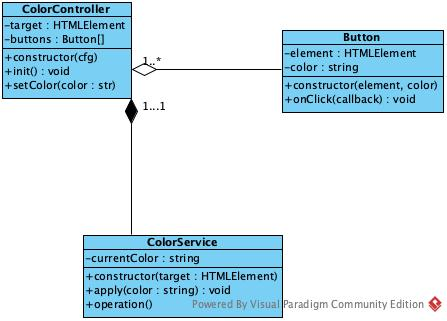
\includegraphics[width=0.7\textwidth]{png/colorButtonPage.jpg}
  \caption{UML Class Diagram for the Refactored Website}
  \label{fig:colorPageClassDiagram}
\end{figure}


\chapter{LaTeX Docker \\
\small{\textit{-- Ivan Farfan, Johan Jaramillo, Ryan Davis}}}
\index{latexdocker} 
\index{Chapter!LaTeXDocker}
\label{Chapter::LaTeXDocker}

\section{Project Layout}
Create a folder with these files:
\begin{minted}[fontsize=\small,breaklines]{text}
.
├── Dockerfile
└── main.tex
\end{minted}

\section{Dockerfile}
This Dockerfile installs TeX Live and sets up a container to compile LaTeX.

\begin{minted}[fontsize=\small,breaklines]{docker}
FROM debian:bookworm-slim
RUN apt-get update && apt-get install -y \
    texlive-latex-base \
    texlive-latex-recommended \
    texlive-latex-extra \
    texlive-fonts-recommended \
    latexmk \
    python3-pygments \
 && apt-get clean && rm -rf /var/lib/apt/lists/*
WORKDIR /data
CMD ["latexmk", "-pdf", "-shell-escape", "main.tex"]
\end{minted}

\section{Build and Run}
\begin{minted}[fontsize=\small,breaklines]{bash}
# Build the Docker image
docker build -t latex-docker .

# Run the container (Linux/macOS)
docker run --rm -v $(pwd):/data latex-docker

# Run the container (Windows PowerShell)
docker run --rm -v ${PWD}:/data latex-docker

# Run the container (Windows CMD)
docker run --rm -v %cd%:/data latex-docker
\end{minted}
\section{Screenshot}
The following screenshot shows the result of compiling our LaTeX document inside
the Docker container.

\begin{center}
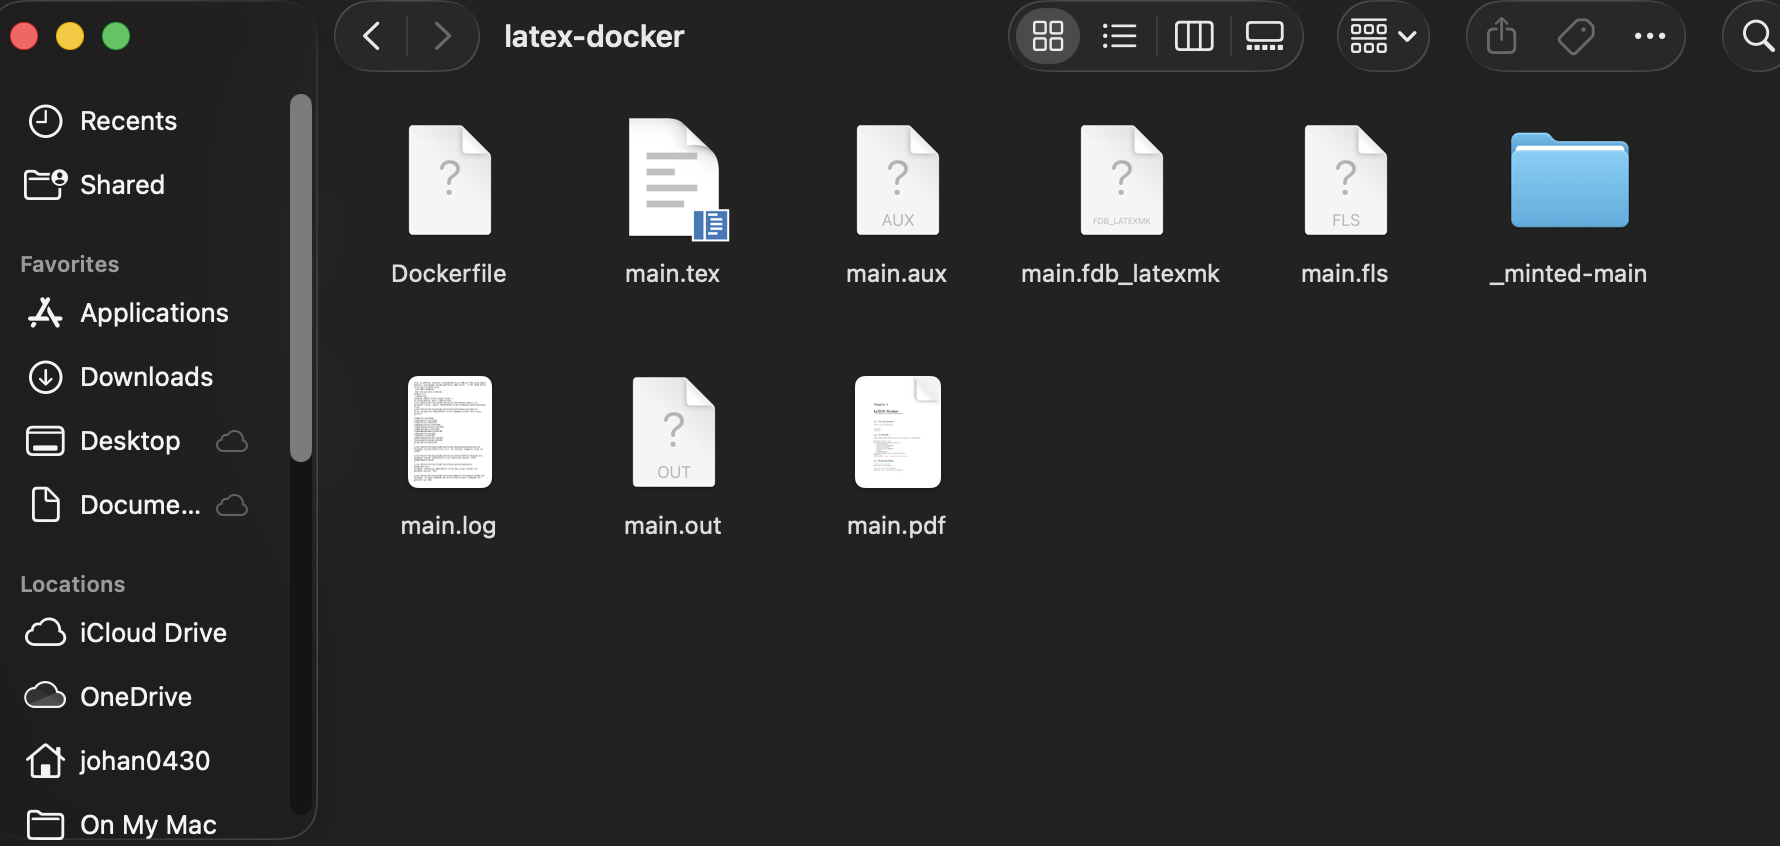
\includegraphics[width=0.9\textwidth]{png/latexdocker.png}
\end{center}


\section{Conclusion}
In this chapter we showed how to use Docker to build a container that can
compile LaTeX documents with TeX Live. The steps included writing a Dockerfile,
setting up the folder structure, and running basic commands to build and run the
container. This setup is similar to how Overleaf works behind the scenes. Even
though our example was simple, it demonstrates how Docker can make LaTeX
compilation consistent and portable across different systems.
\chapter{Bugzilla \\ 
\small{\textit{-- Ivan Farfan, Johan Jaramillo, Ryan Davis}}} 
\index{Bugzilla} \index{Chapter::Bugzilla} \label{Chapter::Bugzilla}
\section{Overview}

For this part of the assignment, Bugzilla, a web-based bug tracking system, was deployed on a DigitalOcean Droplet using Docker containers. Instead of using a prebuilt image with MariaDB included, we configured two separate containers: one running Bugzilla and another running MySQL as the database backend. This approach ensured greater flexibility and easier debugging when dealing with database connection issues.

\noindent
The Bugzilla image used was the official image available on Docker Hub:

\begin{center}
\url{https://hub.docker.com/r/bugzilla/bugzilla-dev}
\end{center}

\section{Configuration Steps}
\subsection{Droplet Setup}
\begin{itemize}
    \item A new DigitalOcean Droplet was created running \texttt{Ubuntu 25.04}.
    \item Docker was installed using the standard package manager:
    \begin{verbatim}
    apt update
    apt install docker.io -y
    \end{verbatim}
    \item Verified that Docker was running correctly with:
    \begin{verbatim}
    systemctl status docker
    \end{verbatim}
\end{itemize}

\subsection{MySQL Container Configuration}
\begin{itemize}
    \item Pulled the MySQL 5.7 image and started the container:
    \begin{verbatim}
    docker run -d \
      --name bugzilla-mysql \
      -e MYSQL_ROOT_PASSWORD=root \
      -e MYSQL_DATABASE=bugs \
      -e MYSQL_USER=bugs \
      -e MYSQL_PASSWORD=bugspass \
      mysql:5.7
    \end{verbatim}
    \item This container served as the database backend for Bugzilla.
    \item Once running, the container could be verified using:
    \begin{verbatim}
    docker ps
    \end{verbatim}
\end{itemize}

\subsection{Bugzilla Container Setup}
\begin{itemize}
    \item Pulled and started the Bugzilla container:
    \begin{verbatim}
    docker run -d \
      --name bugzilla \
      -p 8080:80 \
      --link bugzilla-mysql:mysql \
      bugzilla/bugzilla-dev
    \end{verbatim}
    \item Accessed the Bugzilla container shell:
    \begin{verbatim}
    docker exec -it bugzilla bash
    cd /var/www/html/bugzilla
    \end{verbatim}
    \item Edited the \texttt{localconfig} file to match the MySQL settings:
    \begin{verbatim}
    $db_driver = 'mysql';
    $db_name   = 'bugs';
    $db_user   = 'bugs';
    $db_pass   = 'bugspass';
    $db_host   = 'bugzilla-mysql';
    \end{verbatim}
    \item Ran the initial setup:
    \begin{verbatim}
    ./checksetup.pl
    \end{verbatim}
    \item Created the Bugzilla administrator account when prompted.
\end{itemize}

\subsection{Troubleshooting and Resource Limitations}
During deployment, the initial droplet used was one of the smallest and most affordable DigitalOcean options, which lacked sufficient memory to run both containers simultaneously. This caused the MySQL container to fail with the following error:
\begin{verbatim}
Can't connect to local MySQL server through socket '/var/lib/mysql/mysql.sock'
\end{verbatim}

\noindent
To resolve this issue:
\begin{itemize}
    \item The droplet was temporarily powered off to modify its plan.
    \item It was upgraded to the following configuration:
    \begin{center}
        \begin{tabular}{|l|l|}
        \hline
        Plan Type & Basic Premium Intel \\
        \hline
        vCPUs & 2 \\
        \hline
        Memory & 2 GB \\
        \hline
        Disk & 25 GB \\
        \hline
        Bandwidth & 3 TB \\
        \hline
        Cost & \$24/month (\$0.036/hr) \\
        \hline
        \end{tabular}
    \end{center}
    \item After resizing, both containers were able to start successfully without memory-related errors.
\end{itemize}

\subsection{Apache Restart and Verification}
\begin{itemize}
    \item Restarted Apache within the Bugzilla container:
    \begin{verbatim}
    apachectl restart
    \end{verbatim}
    \item Verified that the Bugzilla web interface was accessible through:
    \begin{center}
    \texttt{http://167.71.179.151:8080/bugzilla/}
    \end{center}
\end{itemize}

\section{Result}
After adjusting the droplet resources and reconfiguring the database settings, Bugzilla successfully initialized and connected to the MySQL backend. The administrator account was created, and the web interface became fully functional and accessible through the public IP and port 8080.

\section{Container Web Access}
To confirm that the Bugzilla instance was properly running and publicly accessible, the container was tested by visiting the droplet’s IP address on port 8080. The Bugzilla login interface loaded successfully, verifying that both the Apache server and MySQL backend were operational.

\begin{figure}[H]
    \centering
    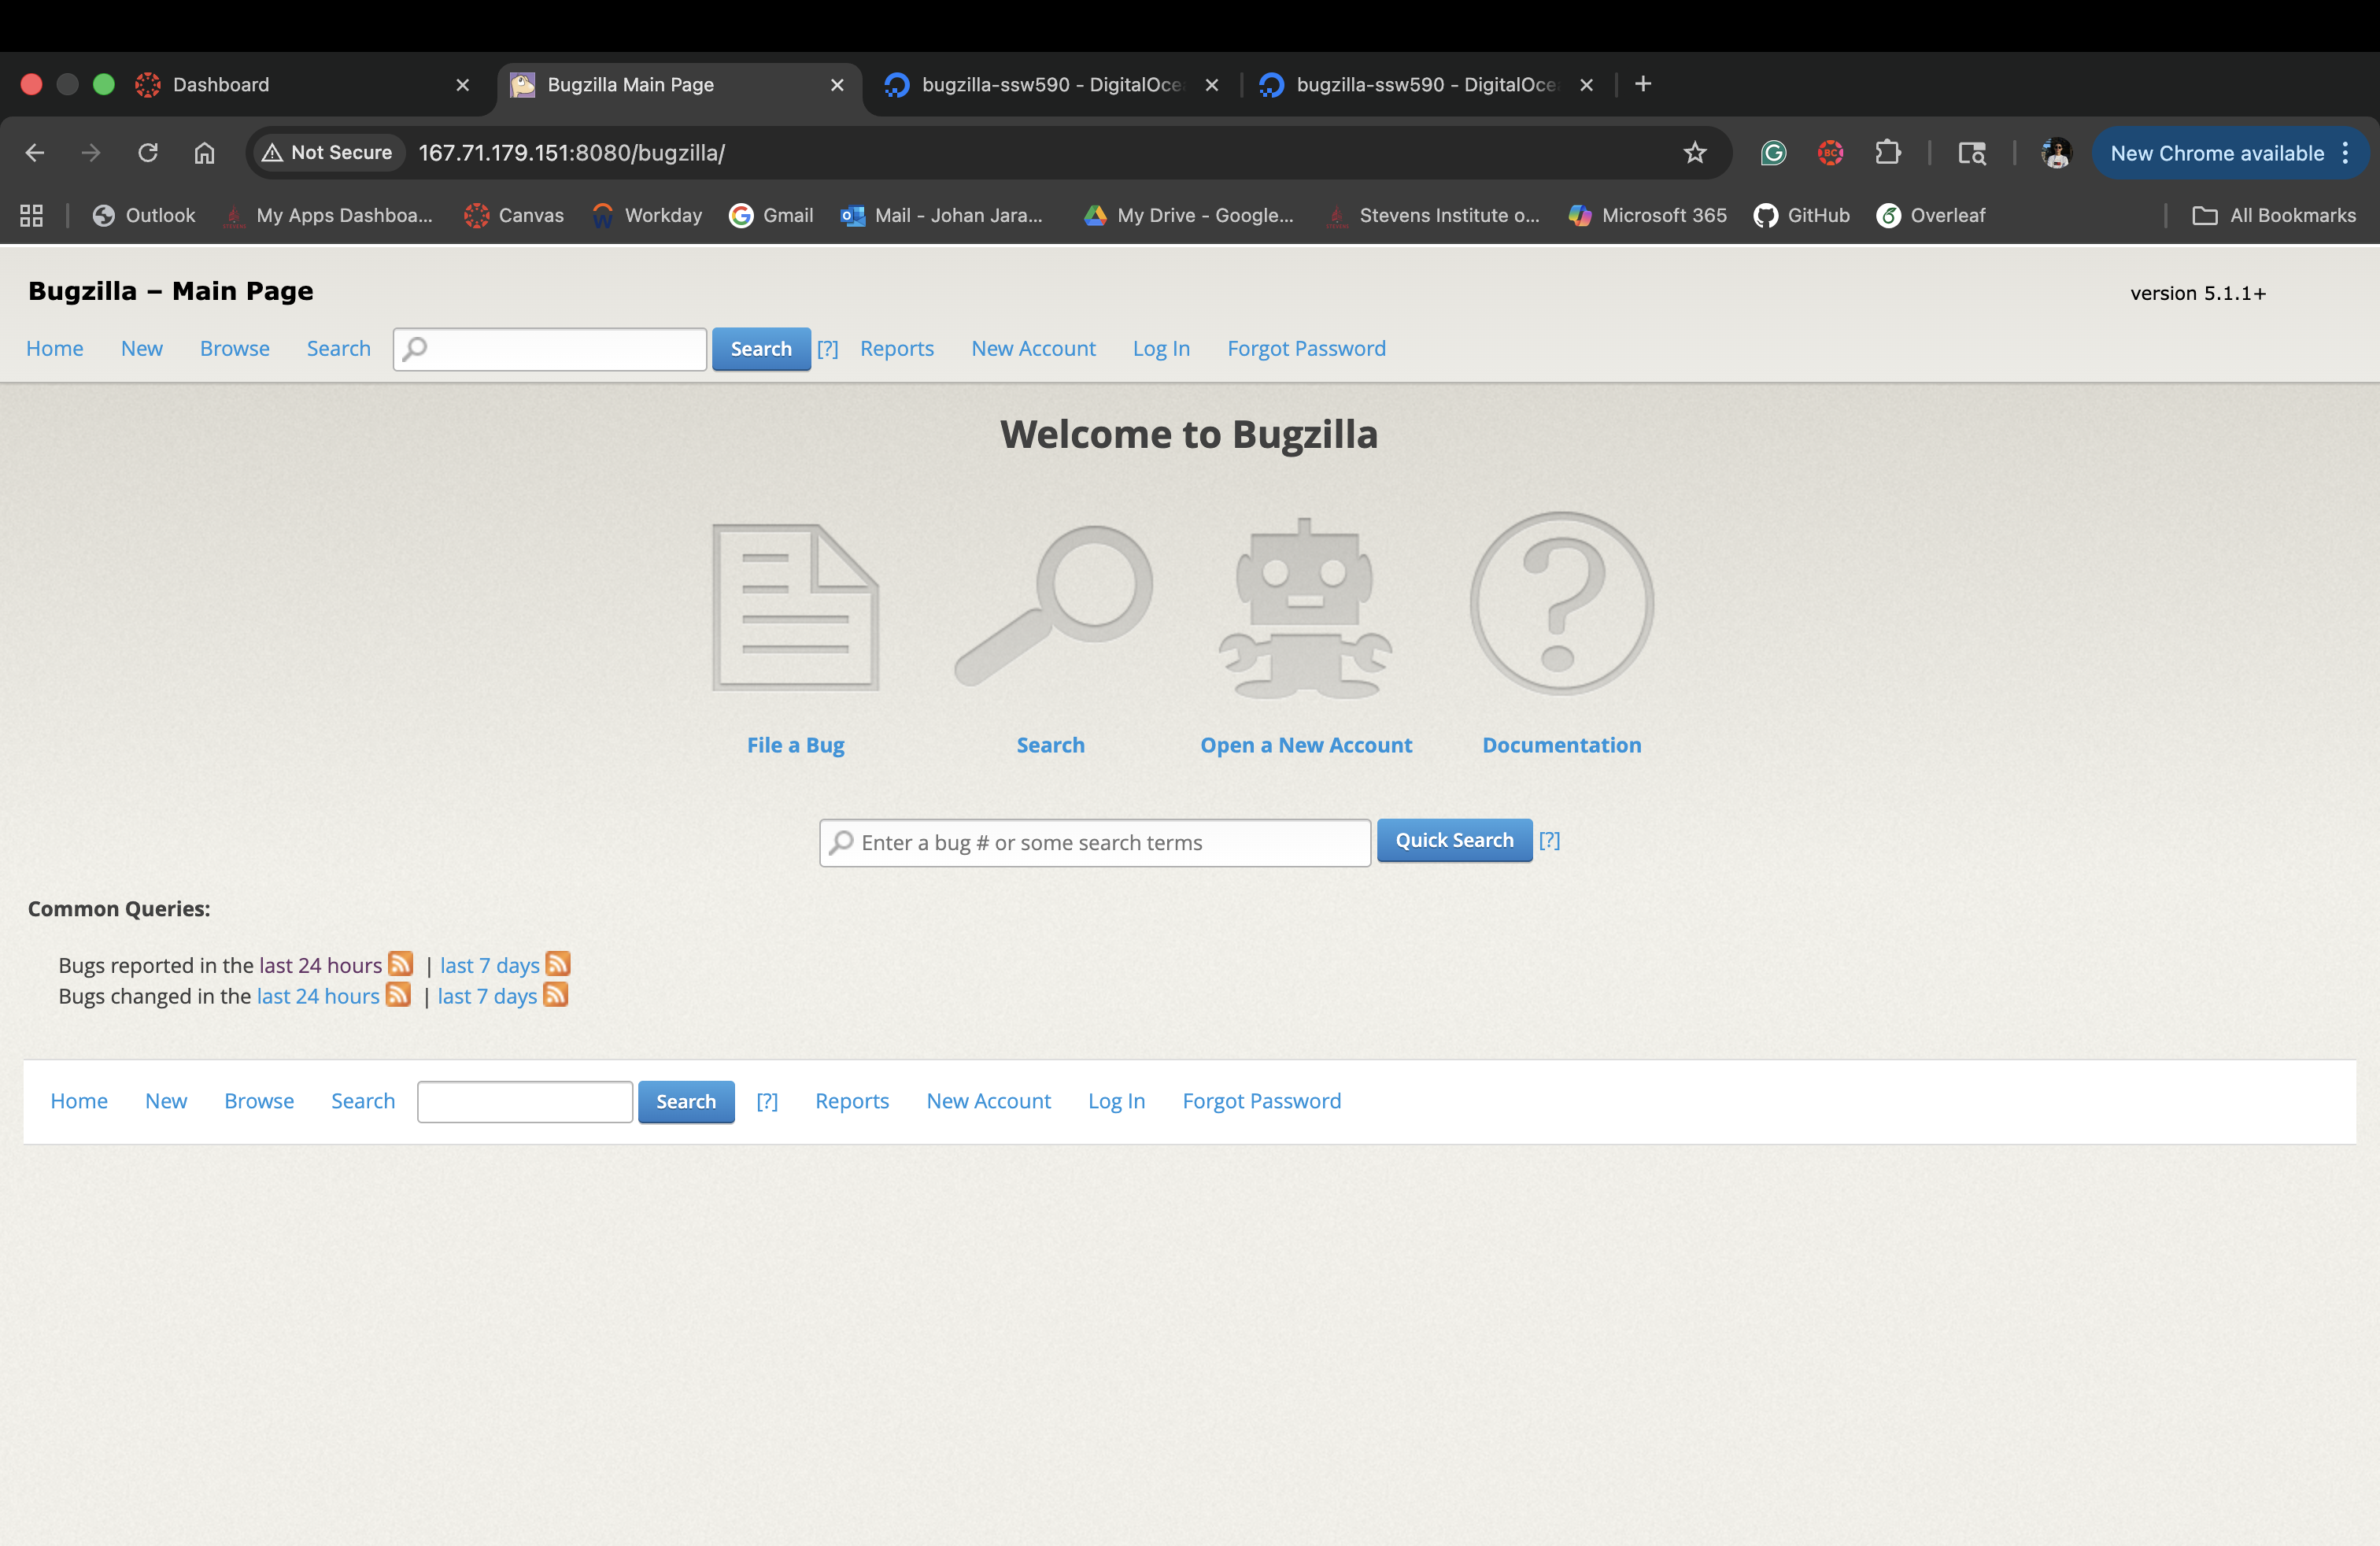
\includegraphics[width=0.9\textwidth]{png/bugzilla.png}
    \caption{Bugzilla web interface confirming successful container deployment on port 8080.}
    \label{fig:bugzilla-port}
\end{figure}

\chapter{Overleaf \\
\small{\textit{-- Ivan Farfan, Johan Jaramillo, Ryan Davis}}}
\index{Overleaf} 
\index{Chapter::Overleaf}
\label{Chapter::Overleaf}

\section{Overview}
For this part of the assignment, Overleaf, a collaborative LaTeX writing platform, was deployed on a DigitalOcean Droplet using Docker containers. The setup required installing Docker and the Docker Compose plugin, verifying the Docker service, and configuring the Overleaf Toolkit container. This approach allowed Overleaf to run directly on port 80, making it accessible through the droplet’s public IP.

\noindent
The Overleaf Toolkit used was obtained from the official GitHub repository:

\begin{center}
\url{https://github.com/overleaf/toolkit}
\end{center}

\section{Configuration Steps}
\subsection{Droplet Setup}
\begin{itemize}
    \item A new DigitalOcean Droplet was created running \texttt{Ubuntu 25.04}.
    \item Docker was installed using the following command:
\begin{minted}[fontsize=\small,breaklines]{bash}
sudo apt install docker.io
\end{minted}

    \item Enabled Docker to automatically start on boot:
\begin{minted}[fontsize=\small,breaklines]{bash}
sudo systemctl enable docker
\end{minted}
\end{itemize}

\subsection{Docker Compose Plugin Installation}
\begin{itemize}
    \item Installed required certificates and tools, then added Docker’s official GPG key:
\begin{minted}[fontsize=\small,breaklines]{bash}
sudo apt-get update
sudo apt-get install ca-certificates curl
sudo install -m 0755 -d /etc/apt/keyrings
sudo curl -fsSL https://download.docker.com/linux/ubuntu/gpg -o /etc/apt/keyrings/docker.asc
sudo chmod a+r /etc/apt/keyrings/docker.asc
\end{minted}

    \item Added Docker’s repository to the Apt sources:
\begin{minted}[fontsize=\small,breaklines]{bash}
echo \
  "deb [arch=$(dpkg --print-architecture) signed-by=/etc/apt/keyrings/docker.asc] \
  https://download.docker.com/linux/ubuntu \
  $(. /etc/os-release && echo "${UBUNTU_CODENAME:-$VERSION_CODENAME}") stable" | \
  sudo tee /etc/apt/sources.list.d/docker.list > /dev/null
sudo apt-get update
\end{minted}

    \item Installed Docker Engine, CLI, and Compose plugin:
\begin{minted}[fontsize=\small,breaklines]{bash}
sudo apt-get install docker-ce docker-ce-cli containerd.io \
docker-buildx-plugin docker-compose-plugin
\end{minted}
\end{itemize}

\subsection{Verifying Docker Status}
\begin{itemize}
    \item Checked that Docker was active and running:
\begin{minted}[fontsize=\small,breaklines]{bash}
sudo systemctl status docker
\end{minted}

    \item The response confirmed a successful installation:
\begin{minted}[fontsize=\small,breaklines]{text}
● docker.service - Docker Application Container Engine
     Loaded: loaded (/usr/lib/systemd/system/docker.service; enabled)
     Active: active (running) since Wed 2025-10-08 19:22:46 UTC
     Main PID: 55151 (dockerd)
     Tasks: 8
     Memory: 43.1M
     CPU: 627ms
\end{minted}
\end{itemize}

\section{Overleaf Toolkit Installation}
\subsection{Preparing the Environment}
\begin{itemize}
    \item Created a directory to hold the container environment:
\begin{minted}[fontsize=\small,breaklines]{bash}
mkdir Overleaf_container
cd Overleaf_container
\end{minted}

    \item Cloned the official Overleaf Toolkit repository:
\begin{minted}[fontsize=\small,breaklines]{bash}
git clone https://github.com/overleaf/toolkit.git
cd toolkit
\end{minted}
\end{itemize}

\subsection{Configuration}
\begin{itemize}
    \item Initialized the configuration files:
\begin{minted}[fontsize=\small,breaklines]{bash}
bin/init
\end{minted}

    \item Edited the Overleaf configuration to listen on all network interfaces:
\begin{minted}[fontsize=\small,breaklines]{bash}
nano config/overleaf.rc
\end{minted}

    \item Updated the following line to allow access from the droplet’s public IP:
\begin{minted}[fontsize=\small,breaklines]{bash}
OVERLEAF_LISTEN_IP=0.0.0.0
\end{minted}
\end{itemize}

\section{Starting Overleaf}
\begin{itemize}
    \item Launched the Overleaf container stack using the toolkit command:
\begin{minted}[fontsize=\small,breaklines]{bash}
bin/up
\end{minted}

    \item This downloaded all required images (MongoDB, Redis, and the Overleaf web app) and automatically started the containers.
    \item Once setup completed, Overleaf was accessible on port 80 of the droplet.
\end{itemize}

\section{Result}
After installation, Overleaf successfully deployed and became accessible through the droplet’s public IP address. All Docker services were active, and the platform functioned correctly for collaborative LaTeX editing.

\section{Container Web Access}
To verify that the Overleaf container was successfully deployed and reachable via the assigned port, the application was accessed through the droplet’s public IP address using a web browser. The interface loaded correctly on port 80, confirming that the Docker service and network configuration were functioning as expected.

\begin{figure}[H]
    \centering
    \includegraphics[width=0.9\textwidth]{png/overleaf.png}
    \caption{Overleaf web interface accessible through port 80 on the droplet.}
    \label{fig:overleaf-port}
\end{figure}


\chapter{Overleaf and Github Integration \\
\small{\textit{-- Ivan Farfan, Johan Jaramillo, Ryan Davis}}}
\index{Overleaf and Github Integration} 
\index{Chapter::Overleaf and Github Integration}
\label{Chapter::Overleaf and Github Integration}

\section{Overview}
For this assignment, we performed the following tasks: getting a domain via the GitHub Student Developer Pack, getting an SSL certificate for our overleaf domain, configure Latex / Overleaf to support all packages, connecting Overleaf to Github for project version control, compiling TEX projects from the command line.

\section{Domain Name}
We decided to register the domain \texttt{ssw590f25.me} using the GitHub Student Developer Pack, which provided a free one-year domain through Namecheap. This allowed us to set up a professional web address for our project with minimal cost and effort. We had to add an A record using the Overleaf \hyperref[Chapter::Hosts]{container droplet IP} as host so that all traffic to the domain gets redirected to the local version of overleaf we're hosting.

\section{SSL Configuration}

To enable HTTPS on our Overleaf container, we installed and configured SSL certificates from Let’s Encrypt using \texttt{certbot}. This ensures secure encrypted communication between users and the server.

\begin{minted}{bash}
apt install python3-certbot-nginx nginx
sudo certbot --nginx certonly
\end{minted}

Once the certificate was obtained, we configured Nginx to serve as a reverse proxy — forwarding client requests to the Overleaf service while handling SSL termination.

\begin{minted}{nginx}
server {
    listen 80;
    server_name overleaf.ssw590f25.me;
    return 301 https://$server_name$request_uri;
}

server {
    listen 443 ssl;
    server_name overleaf.ssw590f25.me;

    ssl_certificate /etc/letsencrypt/live/overleaf.ssw590f25.me/fullchain.pem;
    ssl_certificate_key /etc/letsencrypt/live/overleaf.ssw590f25.me/privkey.pem;

    location / {
        proxy_pass http://localhost:8877;
        proxy_set_header X-Forwarded-For $remote_addr;
    }
}
\end{minted}

Configuring Nginx in this way is crucial because it acts as a reverse proxy—managing secure HTTPS traffic, terminating SSL connections, and forwarding requests to the internal Overleaf container. 

\section{Configuring LaTeX Packages in Overleaf (Container)}

To enable full LaTeX package support inside the Overleaf container, we used the following commands:

\subsection*{Steps}

\paragraph{1) Update \texttt{tlmgr} (TeX Live Manager).}
\begin{minted}{bash}
docker exec sharelatex tlmgr update --self
\end{minted}
\emph{Why:} Brings the package manager itself up-to-date so subsequent installs use the latest metadata.

\paragraph{2) Install the full TeX Live package set.}
\begin{minted}{bash}
docker exec sharelatex tlmgr install scheme-full
\end{minted}
\emph{Why:} \texttt{scheme-full} pulls essentially all TeX Live packages, covering most class/style/font dependencies you’ll encounter.
\textbf{Note:} This took a long time and it's not permanent, it will reset to the basic Latex version if the container is rebuilt.

\section{Connecting Overleaf to GitHub}

We connected our Overleaf instance at \texttt{overleaf.ssw590f25.me} to GitHub to automatically sync compiled project files.

\subsection*{Generating SSH Keys and Configuring Access}

\begin{minted}{bash}
ssh-keygen -t ed25519 -f /root/.ssh/id_ed25519_exports -N "" -C "overleaf-exports"
ssh-keyscan github.com >> /root/.ssh/known_hosts
chmod 600 /root/.ssh/known_hosts
cat /root/.ssh/id_ed25519_exports.pub
ssh -i /root/.ssh/id_ed25519_exports -T git@github.com
\end{minted}

Response:
\begin{verbatim}
Hi IvanFarfan08/Overleaf_Files_SSW590F! You've successfully authenticated, 
but GitHub does not provide shell access.
\end{verbatim}

Configured Git to always use this key:
\begin{minted}{bash}
cat >> /root/.ssh/config <<'EOF'
Host github.com
  User git
  HostName github.com
  IdentityFile ~/.ssh/id_ed25519_exports
  IdentitiesOnly yes
EOF
chmod 600 /root/.ssh/config
\end{minted}

The public key was then added as a deployment key in the GitHub repository.

\subsection*{Creating Export Service}

\begin{minted}{bash}
SRC="/root/Overleaf_container/toolkit/data/overleaf/data/compiles"
DST="/root/overleaf_exports"
REMOTE="git@github.com:IvanFarfan08/Overleaf_Files_SSW590F.git"

sudo apt update
sudo apt install -y git inotify-tools rsync
\end{minted}

Initialized the staging repository:

\begin{minted}{bash}
sudo mkdir -p "$DST"
cd "$DST"
git init -b main
git config user.name  "Overleaf Export Bot"
git config user.email "export@overleaf.local"

cat > .gitignore <<'EOF'
*.aux
*.log
*.out
*.synctex.gz
EOF

git add -A
git commit -m "Initial staging repo"

ssh-keyscan github.com >> /root/.ssh/known_hosts
chmod 600 /root/.ssh/known_hosts
GIT_SSH_COMMAND="ssh -i $KEY -o StrictHostKeyChecking=yes" git push -u origin main
\end{minted}

\subsection*{Watcher Script}

\begin{minted}{bash}
sudo tee /usr/local/bin/compiles-export-push.sh >/dev/null <<'EOF'
#!/usr/bin/env bash
set -euo pipefail

SRC="/root/Overleaf_container/toolkit/data/overleaf/data/compiles"
DST="/root/overleaf_exports"
BRANCH="main"
KEY="/root/.ssh/id_ed25519_exports"

export GIT_SSH_COMMAND="ssh -i $KEY -o StrictHostKeyChecking=yes"

mkdir -p "$DST"

copy_and_commit() {
  local top="$1"
  rsync -a --delete "$SRC/$top/" "$DST/$top/"
  cd "$DST"
  git add "$top"
  if ! git diff --cached --quiet; then
    msg="export: $top @ $(date -u +'%Y-%m-%d %H:%M:%S %Z')"
    git commit -m "$msg"
    git push origin "$BRANCH"
    echo "Pushed: $msg"
  fi
}

DEBOUNCE=5
declare -A last_at

inotifywait -m -r \
  -e close_write,modify,attrib,create,delete,move \
  --format '%w%f' "$SRC" | while read -r path; do
    rel="${path#"$SRC/"}"
    top="${rel%%/*}"
    [ -n "$top" ] || continue

    now=$(date +%s)
    last=${last_at[$top]:-0}
    if (( now - last >= DEBOUNCE )); then
      last_at[$top]=$now
      echo "Detected change in $top"
      copy_and_commit "$top" || echo "Commit/push failed for $top"
    fi
  done
EOF

sudo chmod +x /usr/local/bin/compiles-export-push.sh
\end{minted}

This script continuously monitors the Overleaf compile directory for any changes using
\texttt{inotifywait}. Whenever a project is recompiled, it automatically syncs the updated
subfolder to the local Git staging directory using \texttt{rsync}, commits the changes, and
pushes them to the GitHub repository.  
The \texttt{DEBOUNCE} variable ensures that each subfolder is only pushed once every few
seconds, preventing redundant commits during rapid file writes.

\subsection*{Systemd Service}

\begin{minted}{bash}
sudo tee /etc/systemd/system/compiles-export-push.service >/dev/null <<'EOF'
[Unit]
Description=Export changed Overleaf compiles subfolders to root-owned repo and push
After=network-online.target
Wants=network-online.target

[Service]
Type=simple
User=root
ExecStart=/usr/local/bin/compiles-export-push.sh
Restart=always
RestartSec=2

[Install]
WantedBy=multi-user.target
EOF

sudo systemctl daemon-reload
sudo systemctl enable --now compiles-export-push.service
\end{minted}

The Systemd service runs the watcher script automatically in the background.
It starts on boot, restarts on failure, and ensures continuous syncing between
Overleaf and GitHub. By enabling it with \texttt{systemctl enable --now}, the
service remains active and constantly monitors the compile directory without
manual intervention. The service keeps updating projects (including this one) and is available at \href{https://github.com/IvanFarfan08/Overleaf_Files_SSW590F}{this Github repo}.

\section{Compiling Overleaf Projects from the Command Line}

We found that compiled versions of Overleaf projects are stored in 
toolkit/data/overleaf/data/compiles. 

Each folder in this directory is mapped to a unique \texttt{projectID\_userID} pair.

This means that one can enter the Docker image created in 
\hyperref[Chapter::LaTeXDocker]{Chapter~\ref*{Chapter::LaTeXDocker}} and use the instructions there to compile the project files.  
However, Overleaf automatically generates compiled PDF files for each project, 
and these can already be found in the corresponding folder under the 
\texttt{compiles} directory.

%\appendix
%\chapter{Appendix \\
\small{\textit{-- Author Name}}
\index{appendix} 
\index{Chapter!Appendix}
\label{Chapter::Appendix}}

% makeglossaries dsnManual -- from command prompt.
\clearpage
%\printglossaries


\printnoidxglossaries

\bibliography{bibfile}
%\bibliographystyle{unsrt}
\bibliographystyle{IEEEtran}

\printindex
%\input{dsnManual.idx}
\end{document}
